\subsection{Preprocessing for OCR}

After cutting the license plate, we apply the following preprocessing methods
with OpenCV:
\begin{itemize}
    \item \emph{Normalization:} using the \texttt{cv2.normalize} method.
    \item \emph{Noise removal:} using the
        \texttt{fastNlMeansDenoisingColored} function of OpenCV.
    \item \emph{Erodation:} using a $5 \times 5$ kernel matrix of ones.
    \item \emph{Blur clarification:} for the blur clarification, we used a matrix
        with a value $9$ center surrounded with $-1$ values.
    \item \emph{Adaptive Threshold:} using the \texttt{adaptiveThreshold}
        function of OpenCV. 
\end{itemize}

This results in a much better image for the OCR, converting the image to
grayscale and sharpening the label of the license plate. 

\begin{align*}
    \text{Kernel}_{\text{erodation}}&= 
    \begin{bmatrix}
        1 & 1 & 1\\
        1 & 1 & 1 \\
        1 & 1 & 1
    \end{bmatrix}\\
    \text{Kernel}_{\text{blur clarification}}&= 
    \begin{bmatrix}
        -1 & -1 & -1\\
        -1 & 9  & -1 \\
        -1 & -1 & -1
    \end{bmatrix}
\end{align*}

\begin{figure}
    \begin{subfigure}[b]{.45\textwidth}
        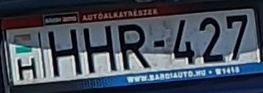
\includegraphics[width=\textwidth]{figures/preprocessbefore1.jpg}
    \end{subfigure}
    \hfill
    \begin{subfigure}[b]{.45\textwidth}
        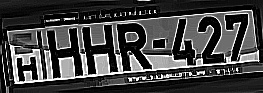
\includegraphics[width=\textwidth]{figures/preprocessafter1.jpg}
    \end{subfigure}
    \hfill
    \\
    \begin{subfigure}[b]{.45\textwidth}
        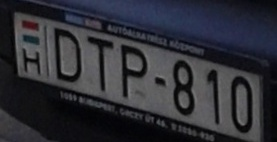
\includegraphics[width=\textwidth]{figures/preprocessbefore2.jpg}
    \end{subfigure}
    \hfill
    \begin{subfigure}[b]{.45\textwidth}
        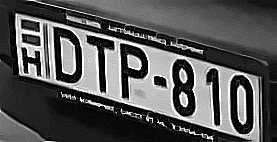
\includegraphics[width=\textwidth]{figures/preprocessafter2.jpg}
    \end{subfigure}
    \hfill
    \\
    \begin{subfigure}[b]{.45\textwidth}
        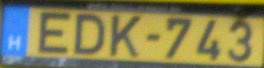
\includegraphics[width=\textwidth]{figures/preprocessbefore3.jpg}
    \end{subfigure}
    \hfill
    \begin{subfigure}[b]{.45\textwidth}
        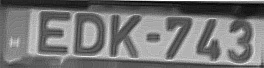
\includegraphics[width=\textwidth]{figures/preprocessafter3.jpg}
    \end{subfigure}
    \hfill
    \caption{Preprocessing results.}
    \label{fig:preprocessing-fig}
\end{figure}
